\documentclass{article}
\usepackage{amsmath,pgf,tikz,array,multirow,tkz-euclide}
\pagestyle{empty}
\raggedright
\usepackage{graphicx,tipa}
\newcommand{\arc}[1]{%
  \setbox9=\hbox{#1}%
  \ooalign{\resizebox{\wd9}{\height}{\texttoptiebar{\phantom{A}}}\cr#1}}
\usepackage[top = 0.5in, left = 1in, bottom = 0.5in, right = 0.5in]{geometry}
\begin{document}

\begin{tabular}{|>{\centering\arraybackslash}m{1.5in}|>{\centering\arraybackslash}m{1.5in}|>{\centering\arraybackslash}m{1.9in}|>{\centering\arraybackslash}m{1.4in}|}
\hline
\textbf{Vertex Location}    &   &   \textbf{Angle Measure}  &   \textbf{Segment Measure}    \\  \hline
Center \newline (equals arc) &   
\vspace{8pt}
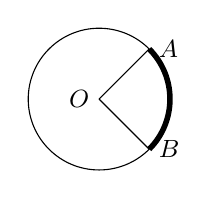
\begin{tikzpicture}[scale=0.9]
    \coordinate (O) at (0,0);
    \draw (O) circle (1cm);
    \coordinate (A) at (45:1cm);
    \coordinate (B) at (-45:1cm);
    \draw (O) -- (A);
    \draw (O) -- (B);
    \node at (O) [anchor = east] {\small $O$};
    \node at (A) [anchor = west] {\small $A$};
    \node at (B) [anchor = west] {\small $B$};
    \draw [line width = 2] (B) arc (-45:45:1cm);
\end{tikzpicture}
&
$m\angle O = m\arc{\textit{AB}}$    &
(the radius)    \\  \hline
Inside \newline (half the sum)   &
\vspace{8pt}
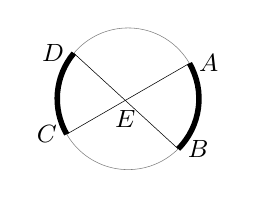
\begin{tikzpicture}[scale=0.9]
    \tkzDefPoint(0,0){O}
    \tkzDefPoint(30:1){A}
    \tkzDrawCircle(O,A)
    \tkzDefPoint(-45:1){B}
    \tkzDefPoint(140:1){D}
    \tkzDefPoint(210:1){C}
    \tkzLabelPoint[right](A){\small $A$}
    \tkzLabelPoint[right](B){\small $B$}
    \tkzLabelPoint[left](D){\small $D$}
    \tkzLabelPoint[left](C){\small $C$}
    \tkzDrawSegments(A,C B,D)
    \tkzInterLL(A,C)(B,D)    \tkzGetPoint{E}
    \tkzLabelPoint[below](E){\small $E$}
    \draw [line width = 2] (B) arc (-45:30:1);
    \draw [line width = 2] (D) arc (140:210:1);
\end{tikzpicture}
&
$m\angle AEB = \frac{1}{2}\left(m\arc{\textit{AB}} + m\arc{\textit{CD}}\right)$
&
$EA \cdot EC = EB \cdot ED$ \\  \hline
\multirow{2}{3.5cm}{On the circle \newline (half the arc)}    &
\vspace{8pt}
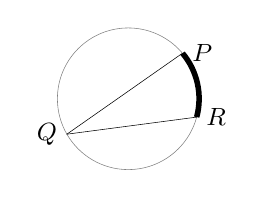
\begin{tikzpicture}[scale=0.9]
    \tkzDefPoint(0,0){O}
    \tkzDefPoint(40:1){P}
    \tkzDrawCircle(O,P)
    \tkzDefPoint(-15:1){R}
    \tkzDefPoint(210:1){Q}
    \tkzDrawSegments(Q,P Q,R)
    \tkzLabelPoint[right](P){\small $P$}
    \tkzLabelPoint[right](R){\small $R$}
    \tkzLabelPoint[left](Q){\small $Q$}
    \draw [line width = 2] (R) arc (-15:40:1);
\end{tikzpicture}
&
$m\angle Q = \frac{1}{2}\left(m\arc{\textit{PR}}\right)$  &  \\ 
&

\vspace{0.25in}
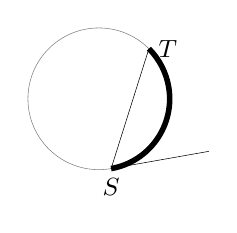
\begin{tikzpicture}[scale=0.9]
    \tkzDefPoint(0,0){O}
    \tkzDefPoint(45:1){T}
    \tkzDrawCircle(O,T)
    \tkzDefPoint(-80:1){S}
    \tkzDrawSegment(S,T)
    \tkzLabelPoint(S){\small $S$}
    \tkzLabelPoint[right](T){\small $T$}
    \tkzDefLine[orthogonal = through S](O,S)
    % \tkzTangent[at=S](O)    
    \tkzGetPoint{h}
    \tkzDrawLine[add=0 and 0.4](S,h)
    \draw [line width = 2] (S) arc (-80:45:1);
\end{tikzpicture}
&
$m\angle S = \frac{1}{2}\left(m\arc{\textit{TS}}\right)$  &  \\ \hline

\multirow{3}{3.5cm}{Outside the circle \newline (half the difference)}    &    
\vspace{8pt}
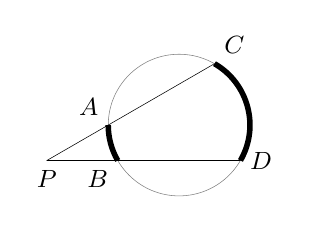
\begin{tikzpicture}[scale=0.9]
    \tkzDefPoint(0,0){O}
    \tkzDefPoint(60:1){C}
    \tkzDefPoint(-30:1){D}
    \tkzDefPoint(180:1){A}
    \tkzDefPoint(210:1){B}
    \tkzDrawCircle(O,C)
    \tkzLabelPoint[above right](C){\small $C$}
    \tkzLabelPoint[right](D){\small $D$}
    \tkzLabelPoint[above left](A){\small $A$}
    \tkzLabelPoint[below left](B){\small $B$}
    \tkzInterLL(C,A)(D,B)   \tkzGetPoint{P}
    \tkzDrawSegments(C,P D,P)
    \tkzLabelPoint[below](P){\small $P$}
    \draw [line width = 2] (D) arc (-30:60:1);
    \draw [line width = 2] (B) arc (210:180:1);
\end{tikzpicture}
&   
$m\angle P = \frac{1}{2}\left(m\arc{\textit{CD}}-m\arc{\textit{AB}}\right)$
&
$PA \cdot PC = PB \cdot PD$ \\  
&
\vspace{0.25in}
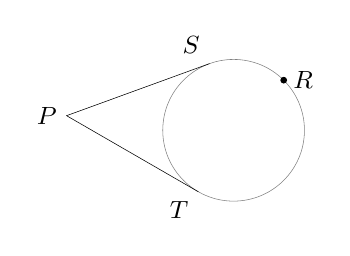
\begin{tikzpicture}[scale=0.9]
    \tkzDefPoint(0,0){O}
    \tkzDefPoint(45:1){R}
    \tkzDefPoint(110:1){S}
    \tkzDefPoint(240:1){T}
    % \tkzDefPoint(170:1.5){P}
    \tkzDefLine[orthogonal = through S](O,S)
    \tkzGetPoint{a}
    \tkzDefLine[orthogonal = through T](O,T)
    \tkzGetPoint{b}
    \tkzInterLL(S,a)(T,b)
    \tkzGetPoint{P}
    \tkzDrawCircle(O,R)
    \tkzLabelPoint[above left](S){\small $S$}
    \tkzLabelPoint[below left](T){\small $T$}
    \tkzDrawPoint[fill=black](R)
    \tkzLabelPoint[right](R){\small $R$}
    \tkzDrawSegments(P,S P,T)
    \tkzLabelPoint[left](P){\small $P$}
\end{tikzpicture}
&
$m\angle P = \frac{1}{2}\left(m\arc{\textit{SRT}}-m\arc{\textit{ST}}\right)$
&
$PS = PT$   \\
&
\vspace{0.25in}
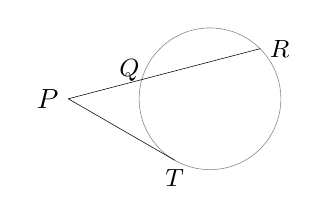
\begin{tikzpicture}[scale=0.9]
    \tkzDefPoint(0,0){O}
    \tkzDefPoint(45:1){R}
    \tkzDefPoint(240:1){T}
    \tkzDefPoint(180:2){P}
    \tkzDrawCircle(O,R)
    \tkzLabelPoint[right](R){\small $R$}
    \tkzDrawSegment(R, P)
    \tkzLabelPoint[below](T){\small $T$}
    % \tkzTangent[from = P](O,T)
    \tkzDefLine[orthogonal = through P](O,T)
    \tkzGetPoint{g}
    \tkzDrawLine[add = 0 and 0](P,T)
    \tkzInterLC(P,R)(O,R)   \tkzGetPoint{Q}
    \tkzLabelPoint[above left, xshift=0.25cm, yshift=0.55cm](Q){\small $Q$}
    \tkzLabelPoints[left](P)
\end{tikzpicture}
&
$m\angle P = \frac{1}{2}\left(m\arc{\textit{RT}}-m\arc{\textit{QT}}\right)$
&
$TP \cdot TP = PR \cdot PQ$   \\[10pt]    \hline
\end{tabular}
			


\end{document}